\lab{Algorithm}{Pseudorandom Number Generators}{Pseudorandom Number Generators}
\label{Ch:PRNG}

\objective{This section teaches about how to build pseudorandom number generators and the differences between the different kinds of PRNGs}

\section*{Random Numbers}

%Lab \ref{PRNG}

Lotteries, most board games, and statistics need random numbers. In real life, we roll dice, take balls out of a bag, or spin a wheel. In order to solve this problem on a computer we have too options. Computers are by their nature deterministic, meaning that they do what they are told. So the problem is how to generate random numbers on computers. We can have a device measure a random process such a device that measures thermal noise or a Geiger counter. But often those are too slow and quite expensive. What is used most oftened is psuedorandom number generators (PRNGs). The numbers are not truly random, but they are based on a complex formula that makes them look ``random." Another thing is that these generators have to be fast for their aplication. So you have to have something that is fast and looks random.

There are many different algorithms for developing psuedorandom numbers. Robert R. Coveyou titled an article ``The generation of random numbers is too important to be left to chance." There has been much study about different PRNGs. This lab will cover two of them: Linear Congruiental Generator and Mersenne Twister.

\section*{Linear congruential genterators}

One of the oldest of these is the Linear Congruiental Generator (LCG). The Generator is defined by the recurrence relation:
$X_{n+1}=(a*X_n + c)$ mod $m$ where

\begin{itemize}
\item[] $X$ is a sequence of pseudorandom values, and
\item[] $m$, $0<m$ is the modulus
\item[] $a$, $0<a<m$ is the multiplier
\item[] $c$, $0\leq c<m$ is the increment
\item[] $X_0$, $0\leq X_0 <m$ is the seed
\end{itemize}


each of these are interger constansts.



\begin{problem}
Write a LCG that produces a number an array of psuedorandom numbers between $0.0$ and $1.0$. Let the arguments be size of array and let a,c,mod,and seed be optional arguments. I recommend $a=1103515245$, $c=12345$, $m=2^{31}-1$, and $seed=4329$ as the defualt values.
\end{problem}

\begin{problem}
Write a LCG that produces a number an array of psuedorandom numbers of integers between two input arguments. Do it by calling your agorithm from problem one and mutiplying it by the values and casting the array as as int using the .astype() function. Let the arguments be size of array and the two intergers. Let a,c,mod,and seed continue to be optional arguments.
\end{problem}

One easy way to ``see" if your generator is random is to look at a bitmap of the output. In python, use the plt.imshow() function to see a bitmap of the array produced by your LCG. Resize your output to be $512 \times 512$. 

\begin{figure}[H]
%\begin{center}
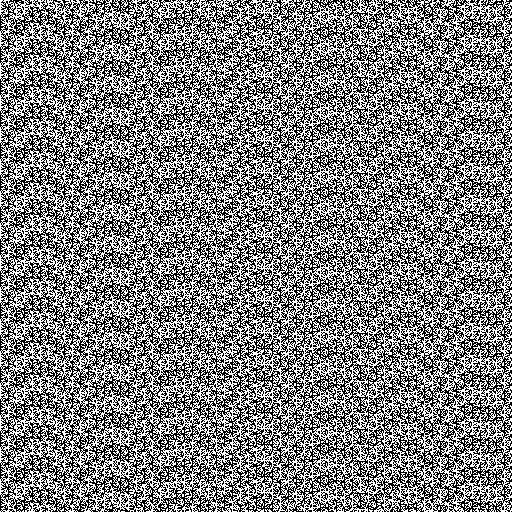
\includegraphics[scale = .4]{PRNG1.jpg}
\caption{The bitmap with $a=25214903917$, $c=11$, $m=2^{48}$. As you can see there is a definite pattern}
%\end{center}
\end{figure}

\begin{problem}
For what values of $a$, $c$, and $m$ does your LCG have a definite pattern.
\end{problem}

This method is not rigorist. There are several ways to test the randomness of your output. 

The length over with your random number generator repeats is called the period. The period is at most m, but it may be shorter based on the values of a and c.
 
According to the Hull-Dobell Theorem (find a source, used wikipedia), The LCG will only have a full period if and only if, 
1. $c$ and $m$ are relatively prime,
2. $a-1$ is divisible by all prime factors of $m$,
3. $a-1$ is a multiple of 4 if $m$ is a multiple of 4

\begin{problem}
Test values of $a$,$c$, and $m$ that fit these requirements. 
\end{problem}

This algorithm is used to generate random numbers in Java, C++ and other places.

\section*{Mersenne Twister and Bitwise operations}


All numbers can be represented in bits as a base two number. Computers are optimized to work with numbers in that manner. There are operations that work on the the bit representation of the two number. These are XOR, OR, and AND. 

AND - if both numbers have a 1 in the ith place then the ith place is 1. Otherwise the ith place is 0.

OR - if one or both numbers have a 1 in the ith place then the ith place is 1. Otherwise the ith place is 0.

XOR - if only one of the two numbers has a 1 in the ith place then the ith place is 1. If both or neither of the numbers has a 1 in the ith place, the ith place is 0.

In addition you can shift the bitwise number over anumber of values. For example, shifting 10100 to the right by one yields 1010 and shifting it to the left by one yields 101000. This can be done by $\ll$ and $\gg$ in python. 


The mersenne twister PRNG does a series of these operations to generate random numbers. the Random class in python uses the mersenne twister algorithm. 

\begin{problem}
Look at the bitmap of output of sp.rand(512,512). Can you see any patterns?
\end{problem}

\begin{problem}
Analyse the first of 10,000 outputs of the random class. Can you see a period?
\end{problem}
